\documentclass{report}
\pagestyle{headings}
\usepackage{url}
\usepackage[dvips]{graphicx}

\author{Geoff Lawler \url{<geoff.lawler@cobham.com>}}
\title{{\bf Watcher Improvments Project}\\Wrapup Report FY08}
% \subtitle{The Search for Spock}

\begin{document}
\maketitle

\renewcommand*\thesection{\arabic{section}}

\section{Introduction}

``The Watcher'' is a MANET visualization tool that allows researchers to visualize the locations and states of nodes in an emulated MANET environment. 
Figure ~\ref{fig:oldWatcher} (page \pageref{fig:oldWatcher}) shows the watcher tool at the start of the improvements project. Figures ~\ref{fig:legWatcherGUI} (page \pageref{fig:legWatcherGUI}) and ~\ref{fig:watcherWithBackground}
(page \pageref{fig:watcherWithBackground}) show the watcher towards the end of the contract. Note that the GUI is now in a window and contains user interface elements such as buttons, menuns, and playback
mechanism. Becauseof the work done on the watcher architecture, it is now possible to have multiple distincy GUIs displaying the same (live or recorded) data 
set at the same time. Figure ~\ref{fig:ogreWatcherGUI} (page \pageref{fig:ogreWatcherGUI}) shows the first cut of a new game-engine based GUI that can be used alone or in tandem with the original watcher GUI. 
\\\\
{\bf something about the old watcher, ARL wanting to improve it, etc. }
\\\\
Below are three sections that give an overview of the work done in the last year on the watcher improvments project. First
is the work accomplished - what was done and why. This is followed by a section on lessons learned from the work done. What is now known 
that was not known then? What would be done differently if given the chance? The final section gives a recommendation on future directions
for the project. Where the watcher system may go and how it will get there. 

\section{Work Performed}

\subsection{Watcher Improvments}
The main watcher GUI had many updates and fixes applied in the first half on the contract. This portion of the time was focused on updatin the GUI to 
support usability and display features for the Army Science Conference in Decemeber. Thus the focus was on modifying the existing code base - fixing bugs, 
and adding features requested by ARL. The last six months of the contract focused much more on the new architecture, full ``TiVO'' mode, and removing 
the reliance on the hierarchy daemons as a transport mechanism. The second half on the contract saw a large amount of code written, new GUIs developed, and 
a near complete rewrite of the existing watcher GUI. 

Here is a list of updates and bug fixes applied in the first half of the contract.

\begin{itemize}
\item Wrapped the OpenGL window in a Qt window, giving us modern GUI widgets. 
\item Use mouse to control movement in the main watcher window.
\item More moduluar logging. Good for debugging and general system performance.
\item Graphcial primatives in watcher window are 3d. Can toggle between 3d and 2d via a menu.
\item Added ability to load a background image into main watcher GUI window and place it as needed via the mouse.
\item Watcher GUI saves state to human readable configuration file on exit. This file is also read on start and watcher honors the 
settings fouind there. File can be edited to modify watcher GUI behavior.
\item Test nodes can control how they are represented in the GUI (shape, size, color, flashing, spining, blinking, etc). These representations
are saved in the watcher configuration file.
\item Can use the mouse to select a node in the GUI.
\item Added 2d scrolling graph to watcher GUI. Test nodes send periodic data to the watcher. The watcher saves this information and when 
a user clicks on a node, the data stored by the watcher is displayed. Mulitple test node's data can be displayed at once and the graph
works in real time, as new data comes in, the old data is scrolled off the end of the graph dialog. Multiple types of period data 
supported. (Although the types are hardcoded. In the second half of the project, these were made dyanmic.) See figure \ref{fig:watcherBandwidthGraphDialog} 
for an example snapshot.
\item Background color of the GUI can be changes at runtime. New color is saved in watcher configuration file.
\end{itemize}

The second half of the contract focused on a new watcher architecture, designed to support full ``TiVO'' mode, fully dynamic system, removing reliance
on hieraxhy daemons as a transport mechanism. Below is a list of highlights from this half of the project.

\begin{itemize}
\item Wrote new watcher messaging system including message parsing, protocols, and message formats from scratch. 
\item Split message handling, message playback, and message caching from graphical represenation. Architecture now
supports a single daemon and multiple different GUIs. 
\item Watcher daemon now uses database to store messages for playback instead of binary blob file format. This allows
flexibility and the abililty of third-party applications to process watcher data. 
\item Rewrote all network code, creating the watcher daemon and removing GUI reliance on hierarchy. Network functionality is now
much more scalable. 
\item Wrote proof of concept watcher GUI based on the Object-Oriented Graphical Rendering Engine (OGRE). See figure \ref{fig:ogreWatcherGUI} for a 
screen shot. 
\item The watcher GUI now supports fully dynamic layers and graph data. No layer or graph data is hardcoded in the watcher system, all 
the layer and graph data is fed directly from test nodes and handled in the GUI in a simple and systematic way.
\item Investigated use of Google Earth for a watcher system GUI. It appears feasiable. 
\item Investigated The Delta-3D game eninge as the basis of a new watcher GUI. Wrote proof of concept application. 
\end{itemize}


\subsection{New Architecture}

The watcher architecture was redesigned and abstract to promote flexibility and extensibility. Divorcing the record 
capability from the display mechanism allowed us to easily add full "TiVO" capability and the ability to have mulitple 
GUIs with independent views into the same dataset. One reseacher can view a testrun which focuses on a single node of region, 
pausing and fast-forwarding a single section of the playing field while another researcher can view it all or jump from 
location to location, viewing multiple different layers of the dataset. See figure \ref{fig:watcherArch.eps} for a diagram 
of the new architecture.

Abstracting the layer concept allows the researcher to add layers dynamically at runtime. For example, 
if a researcher notices a problem with bandwidth usage, he or she can easily write a new test node daemon that 
adds a new ``bandwidth'' layer to the dataset. This new layer shows up in the GUI and can be toggled as needed. 
Compare this to the old watcher which had a fixed, hardcoded set of layers regardless of the components of the test
of the researches needs. The old watcher always had a ``wormhole attacks'' layer even if the test did not 
contain the wormhole detector or even anything wormhole related at all. 

Another benfit to the new architecture is that the system is much more dynamic. The old watcher needed to know all the addreses of all the nodes
on the testbed. This information was even needed when a session was played back. The new system is much more passive - any node can connect and 
send or request data at any time. 

\begin{figure}
\label{fig:oldWatcher}
\centering
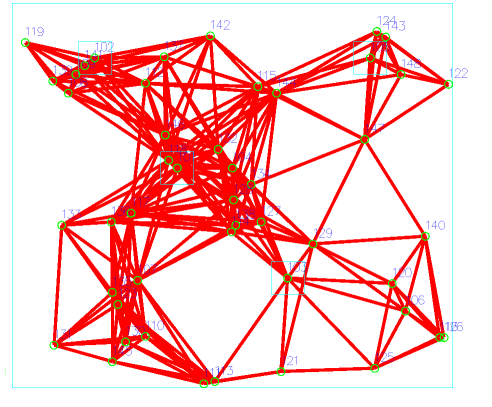
\includegraphics[width=0.5\textwidth]{oldWatcher.eps}
\caption{Watcher at start of project}
\end{figure}

\begin{figure}
\label{fig:legWatcherGUI}
\centering
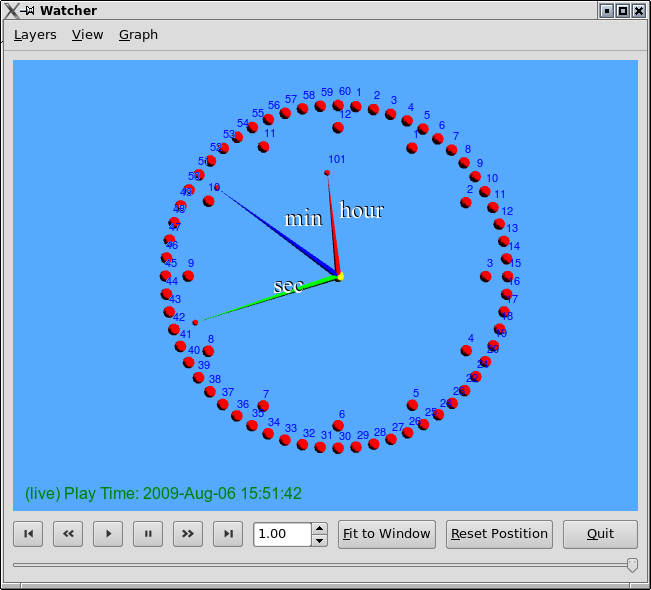
\includegraphics[width=0.8\textwidth]{legWatcherGUI.eps}
\caption{``Legacy Watcher'' at end of project. Note user interface widgets.}
\end{figure}

\begin{figure}
\label{fig:watcherWithBackground}
\centering
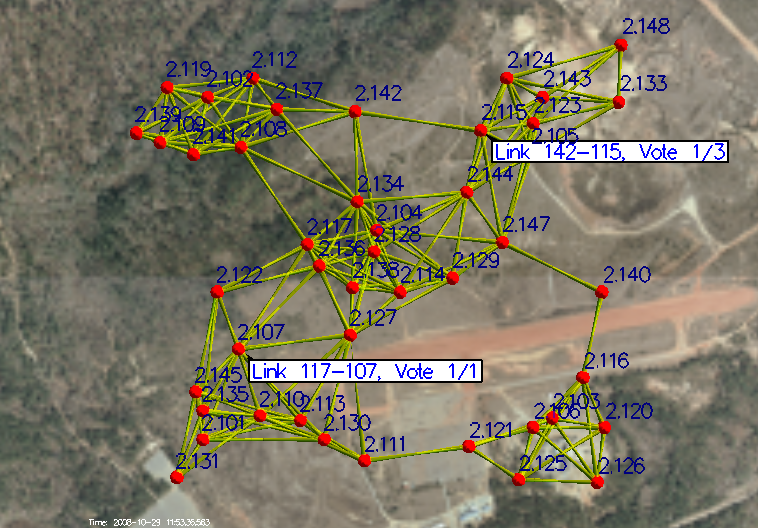
\includegraphics[width=0.8\textwidth]{watcherWithBackground.eps}
\caption{``Legacy Watcher'' showing background and 3D primitives}
\end{figure}

\begin{figure}
\label{fig:ogreWatcherGUI}
\centering
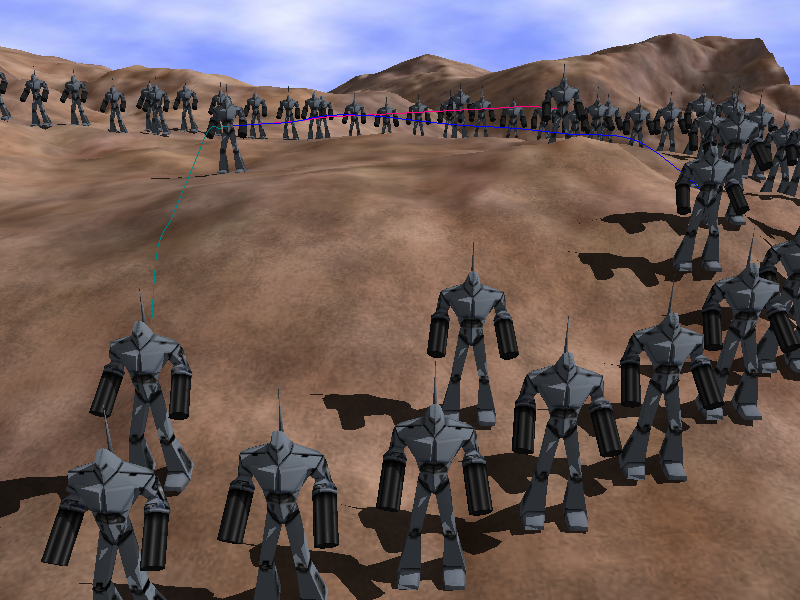
\includegraphics[width=0.8\textwidth]{ogreWatcherGUI.eps}
\caption{First cut at game engine-based watcher GUI. The watcher of the future?}
\end{figure}

\begin{figure}
\label{fig:watcherBandwidthGraphDialog}
\centering
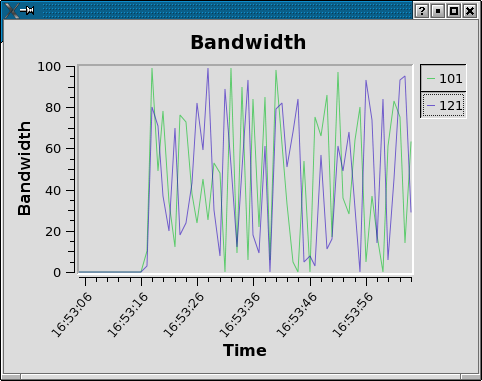
\includegraphics[width=0.8\textwidth]{watcherBandwidthGraphDialog.eps}
\caption{Example of 2d scrolling graph in ``legacy watcher''}
\end{figure}

\section{Lessons Learned}
We learned a lot of stuff, like totally.

\section{Recommendations for Future Work}
We should do some cool stuff in the future, like totally. 

\end{document}


